\documentclass[conference]{IEEEtran}
\IEEEoverridecommandlockouts
% The preceding line is only needed to identify funding in the first footnote. If that is unneeded, please comment it out.
%Template version as of 6/27/2024
\usepackage{amsmath,amssymb,amsfonts}
\usepackage{algorithmic}
\usepackage{graphicx}
\usepackage{textcomp}
\usepackage{xcolor}
\usepackage{hyperref}
\usepackage{url}
\def\BibTeX{{\rm B\kern-.05em{\sc i\kern-.025em b}\kern-.08em
    T\kern-.1667em\lower.7ex\hbox{E}\kern-.125emX}}
\begin{document}

\title{US Bank Loan Portfolio Analytics Using Federal Reserve Regulatory Balance Sheet Filings: Methods, Trends, and Research Directions
}

\author{\IEEEauthorblockN{Venkat Chandrasekar Subramaniam}
\IEEEauthorblockA{\textit{DB Global Technology} \\
\textit{Deutsche Bank}\\
Cary, USA \\
venka\_t@yahoo.com}

}

\maketitle

\begin{abstract}
This document is a model and instructions for \LaTeX.
This and the IEEEtran.cls file define the components of your paper [title, text, heads, etc.]. *CRITICAL: Do Not Use Symbols, Special Characters, Footnotes, 
or Math in Paper Title or Abstract.
\end{abstract}

\begin{IEEEkeywords}
component, formatting, style, styling, insert.
\end{IEEEkeywords}

\section{Introduction}
As part of its macroprudential and microprudential supervision process mandated post the 2008 Global Financial Crisis, the Federal Reserve requires the Bank Holding Companies(BHCs), Savings and Loan Holding Companies(SLHCs) and Intermediate Holding Companies(IHCs) to file various reports. These reports may be on a daily, monthly , quarterly , annual or on in an as required basis. 

All BHCs, SLHCs and IHCs(called Banks hereon) are required to file the FR Y-9C report on a quarterly basis by banks having assets more than \$ 50 Billion or more.This information is used by the Federal Reserve(Fed) to monitor the health of the banks in between inspections.\cite{Fed9C}

In this paper , we will discuss on the opportunities for analytics given by the vast data provided in the FRY-9C.
\subsection{Role of BHCs in US Credit Market}
     BHCs by virtue of their size provide the much required stability to the banking system. BHCs provide approximately 63\% of the total credit in the US as of 2018 which provide the much needed liquidity to the Credit markets. Also since BHCs are subject to enhanced oversight and so any minor glitches in the performance can attract the attention of regulatory agencies like the Fed.
     
     BHCs also offer the much required diversification since the traditional interest income sources do not offer the required economies of scale for sustainability of banks the size of the BHCs and so BHCs are constantly on the lookout for opportunities to provide risk capital. This activity makes BHCs inherently innovative enabling BHCs to diversify their lending. BHCs lend to diversified obligors like private creditors and also engage in market making and underwriting activities.
     
     All the above make the BHCs systemically important despite their critics saying that the large banks(which were the forefathers of the BHCs) were the cause of the 2008 meltdown.
     
\subsection{Reason for considering the FR Y-9C data for Bank analysis}
       The FR Y-9C provides a rich set of data which is available in public in the Federal Financial Institutions Examination Council(FFIEC) website. While the data is provided on an aggregate basis the data has been provided in such a way as to lend itself to further analysis. Further the FR Y-9C is a report which has been specifically designed for Banks and while banks form 63 \% of the total credit only, they form the bulk of the data required for the analysis for the purpose of this paper. Below, I present some of the reasons choosing FR Y-9C over reports like SEC 10-Q Report or NCUA Call reports.
\subsection{The FRY-9C Vs the SEC 10-Q}

The SEC 10-Q is a quarterly financial report which should be filed by publicly traded companies in the United States.\cite{SEC10Q} The SEC 10-Q need not be filed by privately held companies. While all banks are publicly traded in the US due to the capital requirements post the 2008 Global Financial Crisis, the SEC-10Q has got limitations in the analysis of banks.The SEC 10-Q report is a freeform report in that it does not have a specific structure. Because it does not have a specific structure unlike most of the Fed Reports which have a specific structure with instructions for each data item or MDRM reported.\cite{MDRM}

The SEC 10-Q is also a report which is more generically tailored for generic company financials, which may include banks as well as non banks. Given that this paper is about bank loans, the SEC 10-Q dataset would be too comprehensive for the purposes of this paper and using the SEC 10-Q data will inject considerable extra effort in the process. 

\subsection{The FRY-9C vs the NCUA Call Reports}
The National Credit Union Administration(NCUA) requires all Credit Unions to file comprehensive reports at the level of each loan after is available for public consumption its website. These data dumps provide a wealth of information concerning the invdividual loans lent by each credit union.\cite{NCUA} However since we are interested in the performance of bank loans on an aggregation, we will ignore this dataset for the purposes of this paper. The figure below shows a comparison of the approximate filers for FR Y-9C, SEC 10-Q and the NCUA Call reports. Data taken from \cite{9CCount}, \cite{SECCount},\cite{NCUACount}
\begin{figure}[htbp]
	\centerline{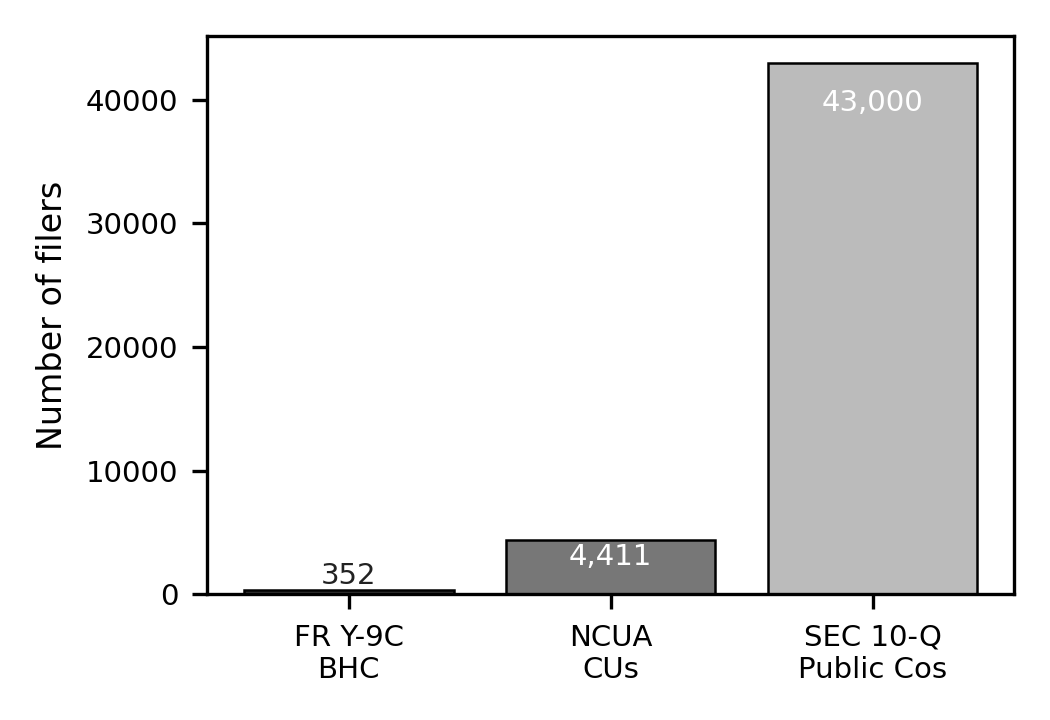
\includegraphics{9C Vs 10-Q Vs NCUA Grayscale.png}}
	\caption{Filer count FR Y-9C, SEC 10-Q, NCUA Call Reports}
	\label{fig}
\end{figure}

\section{History of the FR Y-9C}
Before I delve into the history of FRY-9C, the concept of a BHC must be explained.
\subsection{The BHC Concept}
 The concept of a bank holding company(BHC) came into existence during the mid-1920s with the Fed proposing it in 1927 . The Glass Steagall Act of 1933 provided for the separation of the banking and non banking activities adding more teeth to the principle of BHC. Changes to the construct were made in 1970 when the BHC act was amended. The Dodd Frank Act following the Global Financial Crisis of 2008 created more restictions on BHC while bringing in more banks under the cover of a BHC owing to the ease of supervision under the structure of a BHC.\cite{BHC}

\subsection{The FR Y-9C History}
    According to the Fed in its website, the report started as FRY-9 in 1978. In 1985 report was changed to act as a parallel report to the call reports which are filed in various capacities by banks. For example Deposit taking banks may based on whether they have foreign offices or not need to file the reports of FFIEC-031 or FFIEC-041 which are called the call reports. 
    
    In 1986, the FR Y-9 was split into FR Y-9C (consolidated statement) and FR Y-9LP(Parent company only financial statements) . The threshold for filing the report was changed from \$ 150 million to \$ 3 billion between 2006 and 2018 in various stages. 
    
    The FR Y-9C is required to be filed by BHCs on a quarterly basis in accordance with regulation Y. In 2011, the Dodd Frank Act abolished the Office of Thrift Supervision and SLHCs , except for exempt SLHCs were required to file the FR Y-9C. There was a 2 year phase in period for SLHCs starting Q1 2012 for starting to file FR Y-9C. As per Regulation YY , IHCs of Foreign Banks were also required to file FR Y-9C from 2016.\cite{Fed9C}. The data is summarized as table below
    
    \begin{table}[htbp]
    	\centering
    	\caption{Timeline of FR Y-9C Reporting Requirements\cite{Fed9C}}
    	\begin{tabular}{|p{1.5cm}|p{6cm}|}
    		\hline
    		\textbf{Year} & \textbf{Event} \\
    		\hline
    		1978 & Introduction of FR Y-9 report. \\
    		\hline
    		1985 & Modified to act as parallel to bank Call Reports (FFIEC 031/041). \\
    		\hline
    		1986 & Split into FR Y-9C (Consolidated) and FR Y-9LP (Parent only). \\
    		\hline
    		2006--2018 & Filing threshold raised from \$150M to \$3B. \\
    		\hline
    		2011 & Dodd-Frank: OTS abolished; SLHCs (except exempt) required to file. \\
    		\hline
    		2012--2014 & Two-year phase-in for SLHCs starting Q1 2012. \\
    		\hline
    		2016 & Reg. YY: IHCs of foreign banks required to file. \\
    		\hline
    	\end{tabular}
    \end{table}
\section{FR Y-9C for Bank Loan Analysis}
      The FR Y-9C report is apt for data analysis for the following reasons. The FR Y-9C has got a very well defined MDRM structure where there are rules provided in very minute detail for each MDRM in the report. This makes the report consistent and the reliability of data provided by each bank in each of the MDRM is high. In order to maintain consistency of the data, the Fed publishes a set of Edit Checks as well with the FR Y-9C instructions. A section of these Edit Checks must be satisified in order for banks to even submit the report.These checks and consistent clean data reduce a lot of time spent by researchers in processing the data for their analysis. 
      
      Also the FR Y-9C report data is available for public consumption in the FFIEC website and so considerable time is reduced in obtaining the required permissions for accessing confidential data. This makes data availability faster.
      
      All the above combined with the rich dataset of around 2000 data points or MDRMs provided in FR Y-9C makes it an ideal candidate for Bank data analysis and in specific BHC Loan data analysis.
\section{Purpose of this paper}
This paper attempts to provide a review of the data available in the FR Y-9C report. If the facts provided previously in this paper are taken into consideration and a search is done for scholastic material referencing the FR Y-9C alone, the amount of papers obtained are limited. Given the huge opportunity which lies untapped, this paper attempts to increase the consumption of data from the FR Y-9C for the purposes of research into the behavior of banks and for the economic analyses possible using this very rich dataset provided for free.

Possible areas where FR Y-9C data can be leveraged include usage of FR Y-9C MDRMs as independent variables in the regression equations . Xiangchao et al. \cite{SecRef} use the FR Y-9C data in their investigation to check whether Securitization and CDS have an effect on US Bank Lending . For testing their hypothesis they use the FR Y-9C, they use data from HC-C(Loans and Lease Financing Receivables), HC-R(Risk Weighted Assets) and HC-S(Securitization) to check if CDS and Securitization affect loans growth.

Abdul-Khalik and P.C. Chen use the derivatives data from FRY-9C to examine the impact of derivative trades before and after FAS133 and the use of derivatives by banks to hedge risk in their paper . \cite{der9C}


\section{Brief description of the schedules of FRY-9C}
    The FR Y-9C has got 24 schedules with a number of data points called MDRMs within each schedule. The description of each of the schedules are listed below in the table.
    \begin{table}[htbp]
    	\centering
    	\caption{FR Y-9C Schedules\cite{Fed9C}}
    	\begin{tabular}{|p{1.5cm}|p{6cm}|}
    		\hline
    		\textbf{Schedule} & \textbf{Description} \\
    		\hline
    		HI & Consolidated Income Statement \\
    		\hline
    		HI-A & Changes in Equity Capital \\
    		\hline
    		HI-B & Charge-Offs and Recoveries on Loans and Leases and Changes in Allowances for Credit Losses \\
    		\hline
    		HI-C & Disaggregated Data on the Allowance for Credit Losses \\
    		\hline
    		ISnotes-P & Notes to the Income Statement — Predecessor Financial Items \\
    		\hline
    		ISnotes & Notes to the Income Statement — Other \\
    		\hline
    		HC & Consolidated Balance Sheet \\
    		\hline
    		HC-B & Securities \\
    		\hline
    		HC-C & Loans and Lease Financing Receivables \\
    		\hline
    		HC-D & Trading Assets and Liabilities \\
    		\hline
    		HC-E & Deposit Liabilities \\
    		\hline
    		HC-F & Other Assets \\
    		\hline
    		HC-G & Other Liabilities \\
    		\hline
    		HC-H & Interest Sensitivity \\
    		\hline
    		HC-I & Insurance-Related Underwriting Activities (Including Reinsurance) \\
    		\hline
    		HC-K & Quarterly Averages \\
    		\hline
    		HC-L & Derivatives and Off-Balance Sheet Items \\
    		\hline
    		HC-M & Memoranda \\
    		\hline
    		HC-N & Past Due and Nonaccrual Loans, Leases, and Other Assets \\
    		\hline
    		HC-P & Closed-End 1-4 Family Residential Mortgage Banking Activities \\
    		\hline
    		HC-Q & Financial Assets and Liabilities Measured at Fair Value \\
    		\hline
    		HC-R & Regulatory Capital \\
    		\hline
    		HC-S & Servicing, Securitization, and Asset Sale Activities \\
    		\hline
    		HC-V & Variable Interest Entities \\
    		\hline
    	\end{tabular}
    \end{table}
    
    
    While each schedule might directly or indirectly contribute to the overall loan data the most important schedules which deal with loan data are HC-C Loan and Lease Financing Receivables, HC-N Non Accrual Loans and HC-L Derivatives and Off Balance Sheet items. 
    
    \subsection{HC-C Loans and Lease Financing receivables}
     This section which falls under HC gives details about the Loans and Lease receivables by the bank. Lines 1 to 10 talk about loans post which Lease details kick in. The descriptions of each of the Loan lines is given in Table VII under Appendix.The loans are organized into three sections each section based on Collateral, Borrower and Purpose.
     
     The entire schedule is divided into two columns with one column for the data at a consolidated level and the other for data specifically reported for the domestic offices. Usually MDRMs fall into one or the other category though there are some lines having MDRMs for both categories.
     
     With regard to the individual categories of Collateral, Borrower or Purpose, each MDRM usually falls under one category though the same MDRM falling under two or more categories is also possible. 
     
     \subsubsection{Collateral}
            The MDRMs under this category have the collateral as one of the following
             \begin{table}[htbp]
            	\centering
            	\caption{Collateral Types in HC-C}
            	\begin{tabular}{|p{1.5cm}|p{6cm}|}
            		\hline
            		\textbf{Collateral Type} & \textbf{Lines which fall under category} \\
            		\hline
            		Real Estate & 1 Col A, 1.a.1 Col B, 1.a.2 Col B,1.b,1.c.1,1.c.2.a,1.c.2.b,1.d,1.e.1,1.e.2 \\
            		\hline
            		Unsecured Lending & 6.a,6.b \\
            		\hline
            		Automobile & 6.c \\
            		\hline
            	\end{tabular}
            \end{table}
      
      \subsubsection{Borrower}
            This category has a slight overlap with the type of collateral. Lines under this category are
            \begin{table}[htbp]
            	\centering
            	\caption{Kinds of borrowers with data in HC-C}
            	\begin{tabular}{|p{3.5cm}|p{4cm}|}
            		\hline
            		\textbf{Borrower Type} & \textbf{Lines which fall under category} \\
            		\hline
            		Type of occupier & 1.e.1 ,1.e.2 \\
            		\hline
            		Type of banks & 2.a,2.b \\
            		\hline
            		Farmers & 3 \\
            		\hline
            		Based on address & 4.a,4.b\\
            		\hline
            		Government institutions&7\\
            		\hline
            		Non depository institutions&9.a,9.b.1,9.b.2,9.b.3\\
            		\hline
            		\end{tabular}
            \end{table}
        \subsubsection{Purpose}
             Like the other categories the category of purpose also is split into multiple categories with the type of borrower overlapping with the purpose. Below gives the specific purpose of each of the purpose based detail captured in FR Y-9C
             \begin{table}[htbp]
             	\centering
             	\caption{Purpose Segregation in HC-C}
             	\begin{tabular}{|p{3.5cm}|p{4cm}|}
             		\hline
             		\textbf{Purpose} & \textbf{Lines which fall under category} \\
             		\hline
             		Agriculture & 3. \\
             		\hline
             		Commercial and Industrial Loans & 4.a,4.b \\
             		\hline
             		Personal Expenditure & 6 \\
             		\hline
             		Securities and Financial Transactions & 9.b.1,9.b.3\\
             		\hline
             	\end{tabular}
             \end{table}
            		
            
\section{HC-L Derivatives and off balance sheet items}
    

\section{Plan of the paper}
1. Introduction

Motivation: Why analyze loans at the BHC level?

Role of BHCs in U.S. credit markets.
Importance of supervisory datasets for researchers \& policymakers.

Introduce FR Y-9C (public, quarterly, rich coverage) as the focal dataset.

Contribution of this review: summarizing what loan analytics are possible from FR Y-9C and highlighting research directions.

2. Overview of the FR Y-9C Dataset

Origin and regulatory purpose of FR Y-9C.

Coverage: which institutions file it, reporting frequency.

Loan-related schedules:

HC-C (Loans and Lease Financing Receivables)

HC-N (Past Due and Nonaccrual Loans)

HC-L (Derivatives and Off-Balance Sheet Items)

Related income statement data (HI-B interest income, provisions).

Comparison with other data sources (Call Reports, FR Y-14Q, FFIEC 002).

Strengths and limitations (public availability vs. lack of loan-level detail).

3. Analytical Themes in Loan Portfolio Research

(Each subsection reviews existing methods, stylized facts, and what FR Y-9C enables)

3.1 Loan Composition and Growth
Trends across C\&I, CRE, consumer, agricultural, etc.

Concentration vs. diversification.

Business cycle sensitivity of loan growth.

3.2 Credit Risk and Asset Quality

Nonperforming loans, charge-offs, and provisioning.

Loan loss reserves as a measure of expected credit loss.

Stress-period dynamics (e.g., 2008 crisis, COVID-19).

3.3 Profitability and Loan Pricing

Net interest income and yield analysis.

Loan spreads inferred indirectly from interest income vs. loan balances.

Cross-sectional variation by BHC size/class.

3.4 Capital, Liquidity, and Loan Supply

Interaction between capital adequacy and loan growth.

Liquidity positions and loan expansion/contraction.

Links to macroprudential policies.

3.5 Systemic Risk and Interconnectedness

Concentration of lending across sectors.

Role of large vs. small BHCs in systemic credit provision.

Early warning signals from FR Y-9C aggregates.

4. Methodologies for Loan Analytics

Descriptive/statistical analysis (ratios, growth rates, trend decomposition).

Econometric approaches: panel regressions, dynamic models.

Stress-testing style approaches using FR Y-9C data proxies.

Machine learning applications for risk classification.

Comparisons to loan-level data: What’s possible with aggregate data vs. FR Y-14Q.

5. Policy and Supervisory Applications

How regulators use FR Y-9C to monitor loan quality.

Applications to CCAR/DFAST stress testing.

Use in financial stability monitoring (aggregate lending conditions).

Implications for macroprudential vs. microprudential supervision.

6. Limitations of FR Y-9C for Loan Analytics

Lack of borrower-level detail.

Challenges in sectoral disaggregation (some categories broad).

Time lags and quarterly frequency.

Comparisons with richer supervisory datasets (Y-14Q, confidential Fed datasets).

7. Future Research Directions

Linking FR Y-9C with other datasets (e.g., Call Reports, Y-15 systemic risk data, market data).

Improving loan risk modeling with aggregate vs. micro data.

Cross-country comparisons of supervisory reporting.

Potential role of RegTech and data standardization for future analytics.

8. Conclusion

Summarize key takeaways from the review.

Emphasize FR Y-9C’s role as a public and accessible supervisory dataset.

Call for continued innovation in loan analytics using supervisory filings.
\subsection{Abbreviations and Acronyms}\label{AA}
Define abbreviations and acronyms the first time they are used in the text, 
even after they have been defined in the abstract. Abbreviations such as 
IEEE, SI, MKS, CGS, ac, dc, and rms do not have to be defined. Do not use 
abbreviations in the title or heads unless they are unavoidable.

\subsection{Units}
\begin{itemize}
\item Use either SI (MKS) or CGS as primary units. (SI units are encouraged.) English units may be used as secondary units (in parentheses). An exception would be the use of English units as identifiers in trade, such as ``3.5-inch disk drive''.
\item Avoid combining SI and CGS units, such as current in amperes and magnetic field in oersteds. This often leads to confusion because equations do not balance dimensionally. If you must use mixed units, clearly state the units for each quantity that you use in an equation.
\item Do not mix complete spellings and abbreviations of units: ``Wb/m\textsuperscript{2}'' or ``webers per square meter'', not ``webers/m\textsuperscript{2}''. Spell out units when they appear in text: ``. . . a few henries'', not ``. . . a few H''.
\item Use a zero before decimal points: ``0.25'', not ``.25''. Use ``cm\textsuperscript{3}'', not ``cc''.)
\end{itemize}

\subsection{Equations}
Number equations consecutively. To make your 
equations more compact, you may use the solidus (~/~), the exp function, or 
appropriate exponents. Italicize Roman symbols for quantities and variables, 
but not Greek symbols. Use a long dash rather than a hyphen for a minus 
sign. Punctuate equations with commas or periods when they are part of a 
sentence, as in:
\begin{equation}
a+b=\gamma\label{eq}
\end{equation}

Be sure that the 
symbols in your equation have been defined before or immediately following 
the equation. Use ``\eqref{eq}'', not ``Eq.~\eqref{eq}'' or ``equation \eqref{eq}'', except at 
the beginning of a sentence: ``Equation \eqref{eq} is . . .''

\subsection{\LaTeX-Specific Advice}

Please use ``soft'' (e.g., \verb|\eqref{Eq}|) cross references instead
of ``hard'' references (e.g., \verb|(1)|). That will make it possible
to combine sections, add equations, or change the order of figures or
citations without having to go through the file line by line.

Please don't use the \verb|{eqnarray}| equation environment. Use
\verb|{align}| or \verb|{IEEEeqnarray}| instead. The \verb|{eqnarray}|
environment leaves unsightly spaces around relation symbols.

Please note that the \verb|{subequations}| environment in {\LaTeX}
will increment the main equation counter even when there are no
equation numbers displayed. If you forget that, you might write an
article in which the equation numbers skip from (17) to (20), causing
the copy editors to wonder if you've discovered a new method of
counting.

{\BibTeX} does not work by magic. It doesn't get the bibliographic
data from thin air but from .bib files. If you use {\BibTeX} to produce a
bibliography you must send the .bib files. 

{\LaTeX} can't read your mind. If you assign the same label to a
subsubsection and a table, you might find that Table I has been cross
referenced as Table IV-B3. 

{\LaTeX} does not have precognitive abilities. If you put a
\verb|\label| command before the command that updates the counter it's
supposed to be using, the label will pick up the last counter to be
cross referenced instead. In particular, a \verb|\label| command
should not go before the caption of a figure or a table.

Do not use \verb|\nonumber| inside the \verb|{array}| environment. It
will not stop equation numbers inside \verb|{array}| (there won't be
any anyway) and it might stop a wanted equation number in the
surrounding equation.

\subsection{Some Common Mistakes}\label{SCM}
\begin{itemize}
\item The word ``data'' is plural, not singular.
\item The subscript for the permeability of vacuum $\mu_{0}$, and other common scientific constants, is zero with subscript formatting, not a lowercase letter ``o''.
\item In American English, commas, semicolons, periods, question and exclamation marks are located within quotation marks only when a complete thought or name is cited, such as a title or full quotation. When quotation marks are used, instead of a bold or italic typeface, to highlight a word or phrase, punctuation should appear outside of the quotation marks. A parenthetical phrase or statement at the end of a sentence is punctuated outside of the closing parenthesis (like this). (A parenthetical sentence is punctuated within the parentheses.)
\item A graph within a graph is an ``inset'', not an ``insert''. The word alternatively is preferred to the word ``alternately'' (unless you really mean something that alternates).
\item Do not use the word ``essentially'' to mean ``approximately'' or ``effectively''.
\item In your paper title, if the words ``that uses'' can accurately replace the word ``using'', capitalize the ``u''; if not, keep using lower-cased.
\item Be aware of the different meanings of the homophones ``affect'' and ``effect'', ``complement'' and ``compliment'', ``discreet'' and ``discrete'', ``principal'' and ``principle''.
\item Do not confuse ``imply'' and ``infer''.
\item The prefix ``non'' is not a word; it should be joined to the word it modifies, usually without a hyphen.
\item There is no period after the ``et'' in the Latin abbreviation ``et al.''.
\item The abbreviation ``i.e.'' means ``that is'', and the abbreviation ``e.g.'' means ``for example''.
\end{itemize}
An excellent style manual for science writers is \cite{b7}.

\subsection{Authors and Affiliations}\label{AAA}
\textbf{The class file is designed for, but not limited to, six authors.} A 
minimum of one author is required for all conference articles. Author names 
should be listed starting from left to right and then moving down to the 
next line. This is the author sequence that will be used in future citations 
and by indexing services. Names should not be listed in columns nor group by 
affiliation. Please keep your affiliations as succinct as possible (for 
example, do not differentiate among departments of the same organization).

\subsection{Identify the Headings}\label{ITH}
Headings, or heads, are organizational devices that guide the reader through 
your paper. There are two types: component heads and text heads.

Component heads identify the different components of your paper and are not 
topically subordinate to each other. Examples include Acknowledgments and 
References and, for these, the correct style to use is ``Heading 5''. Use 
``figure caption'' for your Figure captions, and ``table head'' for your 
table title. Run-in heads, such as ``Abstract'', will require you to apply a 
style (in this case, italic) in addition to the style provided by the drop 
down menu to differentiate the head from the text.

Text heads organize the topics on a relational, hierarchical basis. For 
example, the paper title is the primary text head because all subsequent 
material relates and elaborates on this one topic. If there are two or more 
sub-topics, the next level head (uppercase Roman numerals) should be used 
and, conversely, if there are not at least two sub-topics, then no subheads 
should be introduced.

\subsection{Figures and Tables}\label{FAT}
\paragraph{Positioning Figures and Tables} Place figures and tables at the top and 
bottom of columns. Avoid placing them in the middle of columns. Large 
figures and tables may span across both columns. Figure captions should be 
below the figures; table heads should appear above the tables. Insert 
figures and tables after they are cited in the text. Use the abbreviation 
``Fig.~\ref{fig}'', even at the beginning of a sentence.

\begin{table}[htbp]
\caption{Table Type Styles}
\begin{center}
\begin{tabular}{|c|c|c|c|}
\hline
\textbf{Table}&\multicolumn{3}{|c|}{\textbf{Table Column Head}} \\
\cline{2-4} 
\textbf{Head} & \textbf{\textit{Table column subhead}}& \textbf{\textit{Subhead}}& \textbf{\textit{Subhead}} \\
\hline
copy& More table copy$^{\mathrm{a}}$& &  \\
\hline
\multicolumn{4}{l}{$^{\mathrm{a}}$Sample of a Table footnote.}
\end{tabular}
\label{tab1}
\end{center}
\end{table}

\begin{figure}[htbp]
\centerline{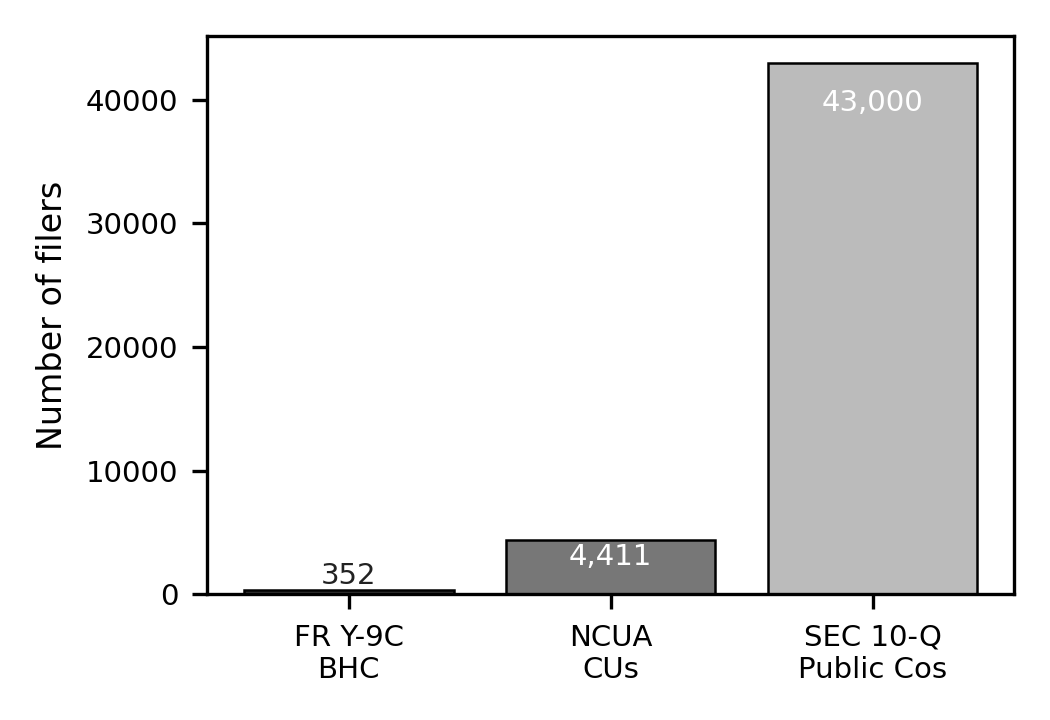
\includegraphics{9C Vs 10-Q Vs NCUA Grayscale.png}}
\caption{Filer count FR Y-9C, SEC 10-Q, NCUA Call Reports}
\label{fig}
\end{figure}

Figure Labels: Use 8 point Times New Roman for Figure labels. Use words 
rather than symbols or abbreviations when writing Figure axis labels to 
avoid confusing the reader. As an example, write the quantity 
``Magnetization'', or ``Magnetization, M'', not just ``M''. If including 
units in the label, present them within parentheses. Do not label axes only 
with units. In the example, write ``Magnetization (A/m)'' or ``Magnetization 
\{A[m(1)]\}'', not just ``A/m''. Do not label axes with a ratio of 
quantities and units. For example, write ``Temperature (K)'', not 
``Temperature/K''.

\section*{Acknowledgment}

The preferred spelling of the word ``acknowledgment'' in America is without 
an ``e'' after the ``g''. Avoid the stilted expression ``one of us (R. B. 
G.) thanks $\ldots$''. Instead, try ``R. B. G. thanks$\ldots$''. Put sponsor 
acknowledgments in the unnumbered footnote on the first page.

\section*{References}

Please number citations consecutively within brackets \cite{b1}. The 
sentence punctuation follows the bracket \cite{b2}. Refer simply to the reference 
number, as in \cite{b3}---do not use ``Ref. \cite{b3}'' or ``reference \cite{b3}'' except at 
the beginning of a sentence: ``Reference \cite{b3} was the first $\ldots$''

Number footnotes separately in superscripts. Place the actual footnote at 
the bottom of the column in which it was cited. Do not put footnotes in the 
abstract or reference list. Use letters for table footnotes.

Unless there are six authors or more give all authors' names; do not use 
``et al.''. Papers that have not been published, even if they have been 
submitted for publication, should be cited as ``unpublished'' \cite{b4}. Papers 
that have been accepted for publication should be cited as ``in press'' \cite{b5}. 
Capitalize only the first word in a paper title, except for proper nouns and 
element symbols.

For papers published in translation journals, please give the English 
citation first, followed by the original foreign-language citation \cite{b6}.


\begin{thebibliography}{00}
\bibitem{Cong1} “Bank Holding Companies: Background and Issues for Congress”, [Online]. Available: \url{https://www.everycrsreport.com/reports/R48291.html#:~:text=Contrary%20to%20traditional%20notions%20that,be%20allowed%20to%20engage%20in.}
\bibitem{Fed9C} “Federal Reserve Board - Reporting Forms.” Accessed: Sept. 06, 2025. [Online]. Available: \url{https://www.federalreserve.gov/apps/reportingforms/Report/Index/FR_Y-9C}
\bibitem{SEC10Q} ``SEC Form 10-Q Instructions''[Online] Available: \url{https://www.sec.gov/files/form10-q.pdf} 
\bibitem{MDRM} “The Fed - Micro Data Reference Manual.” Accessed: Sept. 06, 2025. [Online]. Available: https://www.federalreserve.gov/apps/mdrm/
\bibitem{NCUA} [1] “Credit Union and Corporate Call Report Data | NCUA.” Accessed: Sept. 06, 2025. [Online]. Available: https://ncua.gov/analysis/credit-union-corporate-call-report-data
\bibitem{9CCount} ``Fed Register FRY-9C" [Online] Available : \url{https://public-inspection.federalregister.gov/2024-26707.pdf?1731591951}
\bibitem{NCUACount} “Credit Union Assets, Loans Outstanding and Net Income Increase | NCUA.” Accessed: Sept. 06, 2025. [Online]. Available:\url{ https://ncua.gov/newsroom/press-release/2025/credit-union-assets-loans-outstanding-and-net-income-increase?utm_source=chatgpt.com}
\bibitem{SECCount} “Number of Listed Companies for United States (DDOM01USA644NWDB) | FRED | St. Louis Fed.” Accessed: Sept. 06, 2025. [Online]. Available: https://fred.stlouisfed.org/series/DDOM01USA644NWDB
\bibitem{SecRef} Xiangchao Hao, Qinru Sun, Fang Xie, International evidence for the substitution effect of FX derivatives usage on bank capital buffer, Research in International Business and Finance, 10.1016/j.ribaf.2022.101687, 62, (101687), (2022).
\bibitem{der9C} A. R. Abdel-khalik and P.-C. Chen, “Growth in financial derivatives: The public policy and accounting incentives,” Journal of Accounting and Public Policy, vol. 34, no. 3, pp. 291–318, 2015, doi: https://doi.org/10.1016/j.jaccpubpol.2015.01.002.

 
\bibitem{b10} ``Treatment episode data set: discharges (TEDS-D): concatenated, 2006 to 2009.'' U.S. Department of Health and Human Services, Substance Abuse and Mental Health Services Administration, Office of Applied Studies, August, 2013, DOI:10.3886/ICPSR30122.v2
\bibitem{b11} K. Eves and J. Valasek, ``Adaptive control for singularly perturbed systems examples,'' Code Ocean, Aug. 2023. [Online]. Available: https://codeocean.com/capsule/4989235/tree
\bibitem{BHC} “Bank Holding Companies: Background and Issues for Congress”, [Online]. Available: \url{https://www.everycrsreport.com/reports/R48291.html#:~:text=Contrary%20to%20traditional%20notions%20that,be%20allowed%20to%20engage%20in.}
\bibitem{Fed1}[2] J. Berrospide, F. Cai, S. Lewis-Hayre, and F. Zikes, “Bank Lending to Private Credit: Size, Characteristics, and Financial Stability Implications,” May 2025, Accessed: Aug. 18, 2025. [Online]. Available: https://www.federalreserve.gov/econres/notes/feds-notes/bank-lending-to-private-credit-size-characteristics-and-financial-stability-implications-20250523.html
\bibitem{EAR} A. (Aloke) Ghosh, H. Jarva, and S. G. Ryan, “Bank Regulation/Supervision and Bank Auditing,” European Accounting Review, pp. 1–26, Aug. 2024, doi: 10.1080/09638180.2024.2373207.
\bibitem{NII} M. K. Brunnermeier, G. N. Dong, and D. Palia, “Banks’ Noninterest Income and Systemic Risk,” The Review of Corporate Finance Studies, p. cfaa006, May 2020, doi: 10.1093/rcfs/cfaa006.
\bibitem{Fed2} “FDIC Quarterly - Bank and Nonbank Lending over the past 70 years,” Numb er, vol. 1, 2019.
\end{thebibliography}

\section{Appendix}

\subsection{Appendix I - Line descriptions in HC-C}
\begin{table*}[htbp]
	\centering
	\caption{Loan Categories and Descriptions}
	\begin{tabular}{|p{3cm}|p{12cm}|}
		\hline
		\textbf{Line} & \textbf{Description} \\
		\hline
		1 & Loans secured by real estate. \\
		\hline
		1.a.1 & Construction, land development, and other land loans: 1-4 family residential construction loans. \\
		\hline
		1.a.2 & Construction, land development, and other land loans: Other construction loans and all land development and other land loans. \\
		\hline
		1.b & Secured by farmland. \\
		\hline
		1.c.1 & Secured by 1–4 family residential properties: Revolving, open-end loans secured by 1–4 family residential properties and extended under lines of credit. \\
		\hline
		1.c.2.a & Secured by 1–4 family residential properties: Closed-end loans secured by 1–4 family residential properties — Secured by first liens. \\
		\hline
		1.c.2.b & Secured by 1–4 family residential properties: Closed-end loans secured by 1–4 family residential properties — Secured by junior liens. \\
		\hline
		1.d & Secured by multifamily (5 or more) residential properties. \\
		\hline
		1.e.1 & Secured by nonfarm nonresidential properties — Loans secured by owner-occupied nonfarm nonresidential properties. \\
		\hline
		1.e.2 & Secured by nonfarm nonresidential properties — Loans secured by other nonfarm nonresidential properties. \\
		\hline
		2.a & Loans to depository institutions and acceptances of other banks — To U.S. banks and other U.S. depository institutions. \\
		\hline
		2.b & Loans to depository institutions and acceptances of other banks — To foreign banks. \\
		\hline
		3 Col A & Loans to finance agricultural production and other loans to farmers — Consolidated level. \\
		\hline
		3 Col B & Loans to finance agricultural production and other loans to farmers — Domestic level. \\
		\hline
		4.a & Commercial and Industrial loans — To U.S. addresses (domicile). \\
		\hline
		4.b & Commercial and Industrial loans — To non-U.S. addresses (domicile). \\
		\hline
		4.c & Commercial and Industrial loans — To U.S. addressees and non - US Addresses (domicile). \\
		\hline
		6.a & Loans to individuals for household, family, and other personal expenditures (consumer loans) (includes purchased paper) — Credit cards. \\
		\hline
		6.b & Loans to individuals for household, family, and other personal expenditures (consumer loans) (includes purchased paper) — Other revolving credit plans. \\
		\hline
		6.c & Loans to individuals for household, family, and other personal expenditures (consumer loans) (includes purchased paper) — Automobile loans. \\
		\hline
		6.d & Loans to individuals for household, family, and other personal expenditures (consumer loans) (includes purchased paper) — Other consumer loans (includes single payment, installment, and student loans). \\
		\hline
		7 Col A & Loans to foreign governments and official institutions (including foreign central banks) — Consolidated level. \\
		\hline
		7 Col B & Loans to foreign governments and official institutions (including foreign central banks) — Domestic office level. \\
		\hline
		9.a Col A & Loans to nondepository financial institutions and other loans: Loans to nondepository financial institutions — Consolidated. \\
		\hline
		9.a Col B & Loans to nondepository financial institutions and other loans: Loans to nondepository financial institutions — Domestic offices. \\
		\hline
		9.b.1 Col A & Loans to nondepository financial institutions and other loans: Other loans — Loans for purchasing and carrying securities (secured or unsecured) — Consolidated. \\
		\hline
		9.b.1 Col B & Loans to nondepository financial institutions and other loans: Other loans — Loans for purchasing and carrying securities (secured or unsecured) — Domestic offices. \\
		\hline
		9.b.2 Col A & Loans to nondepository financial institutions and other loans: All other loans (exclude consumer loans) — Consolidated. \\
		\hline
		9.b.2 Col B & Loans to nondepository financial institutions and other loans: All other loans (exclude consumer loans) — Domestic offices. \\
		\hline
		9.b.3 Col A & Loans to nondepository financial institutions and other loans: Loans for purchasing or carrying securities (secured and unsecured) and all other loans — Consolidated. \\
		\hline
		9.b.3 Col B & Loans to nondepository financial institutions and other loans: Loans for purchasing or carrying securities (secured and unsecured) and all other loans — Domestic offices. \\
		\hline
	\end{tabular}
\end{table*}




\vspace{12pt}
\color{red}
IEEE conference templates contain guidance text for composing and formatting conference papers. Please ensure that all template text is removed from your conference paper prior to submission to the conference. Failure to remove the template text from your paper may result in your paper not being published.


\end{document}
